\documentclass[a4paper]{article}

\usepackage{inputenc}
\usepackage[british,UKenglish]{babel}
\usepackage{amsmath}
%\usepackage{titlesec}
\usepackage{color}
\usepackage{graphicx}
\usepackage{fancyref}
\usepackage{hyperref}
\usepackage{float}
\usepackage{scrextend}
\usepackage{setspace}
\usepackage{xargs}
\usepackage{multicol}
\usepackage{nameref}

\usepackage{sectsty}
\usepackage{multicol}
\usepackage{multirow}
\usepackage[procnames]{listings}
\usepackage{appendix}
\usepackage{geometry}
\usepackage{titlesec}

\newcommand\tab[1][1cm]{\hspace*{#1}}
\hypersetup{colorlinks=true, linkcolor=black}
\interfootnotelinepenalty=10000

\newcommand{\cleancode}[1]{\begin{addmargin}[3em]{3em}\texttt{\textcolor{cleanOrange}{#1}}\end{addmargin}}
\newcommand{\cleanstyle}[1]{\text{\textcolor{cleanOrange}{\texttt{#1}}}}


\usepackage[colorinlistoftodos,prependcaption,textsize=footnotesize]{todonotes}
\newcommandx{\commred}[2][1=]{\textcolor{Red}
{\todo[linecolor=red,backgroundcolor=red!25,bordercolor=red,#1]{#2}}}
\newcommandx{\commblue}[2][1=]{\textcolor{Blue}
{\todo[linecolor=blue,backgroundcolor=blue!25,bordercolor=blue,#1]{#2}}}
\newcommandx{\commgreen}[2][1=]{\textcolor{OliveGreen}{\todo[linecolor=OliveGreen,backgroundcolor=OliveGreen!25,bordercolor=OliveGreen,#1]{#2}}}
\newcommandx{\commpurp}[2][1=]{\textcolor{Plum}{\todo[linecolor=Plum,backgroundcolor=Plum!25,bordercolor=Plum,#1]{#2}}}

\def\code#1{{\tt #1}}

\def\note#1{\noindent{\bf [Note: #1]}}

\makeatletter
%% The "\@seccntformat" command is an auxiliary command
%% (see pp. 26f. of 'The LaTeX Companion,' 2nd. ed.)
\def\@seccntformat#1{\@ifundefined{#1@cntformat}%
   {\csname the#1\endcsname\quad}  % default
   {\csname #1@cntformat\endcsname}% enable individual control
}
\let\oldappendix\appendix %% save current definition of \appendix
\renewcommand\appendix{%
    \oldappendix
    \newcommand{\section@cntformat}{\appendixname~\thesection\quad}
}
\makeatother


% "define" Scala
\usepackage[T1]{fontenc}  
\usepackage[scaled=0.82]{beramono}  
\usepackage{microtype} 

\sbox0{\small\ttfamily A}
\edef\mybasewidth{\the\wd0 }

\lstdefinelanguage{scala}{
  morekeywords={abstract,case,catch,class,def,%
    do,else,extends,false,final,finally,%
    for,if,implicit,import,match,mixin,%
    new,null,object,override,package,%
    private,protected,requires,return,sealed,%
    super,this,throw,trait,true,try,%
    type,val,var,while,with,yield},
  sensitive=true,
  morecomment=[l]{//},
  morecomment=[n]{/*}{*/},
  morestring=[b]",
  morestring=[b]',
  morestring=[b]"""
}

\usepackage{color}
\definecolor{dkgreen}{rgb}{0,0.6,0}
\definecolor{gray}{rgb}{0.5,0.5,0.5}
\definecolor{mauve}{rgb}{0.58,0,0.82}

% Default settings for code listings
\lstset{frame=tb,
  language=scala,
  aboveskip=3mm,
  belowskip=3mm,
  showstringspaces=false,
  columns=fixed, % basewidth=\mybasewidth,
  basicstyle={\small\ttfamily},
  numbers=none,
  numberstyle=\footnotesize\color{gray},
  % identifierstyle=\color{red},
  keywordstyle=\color{blue},
  commentstyle=\color{dkgreen},
  stringstyle=\color{mauve},
  frame=single,
  breaklines=true,
  breakatwhitespace=true,
  procnamekeys={def, val, var, class, trait, object, extends},
  procnamestyle=\ttfamily\color{red},
  tabsize=2
}

\lstnewenvironment{scala}[1][]
{\lstset{language=scala,#1}}
{}
\lstnewenvironment{cpp}[1][]
{\lstset{language=C++,#1}}
{}
\lstnewenvironment{bash}[1][]
{\lstset{language=bash,#1}}
{}
\lstnewenvironment{verilog}[1][]
{\lstset{language=verilog,#1}}
{}



\lstset{frame=, basicstyle={\footnotesize\ttfamily}}
\geometry{left=3.17cm,right=3.17cm,top=2.54cm,bottom=2.54cm}
\newpagestyle{main}{            
    \sethead{左页眉}{中页眉}{右页眉}     %设置页眉
    \setfoot{左页脚}{\thepage}{右页脚}      %设置页脚,可以在页脚添加 \thepage  显示页数
    \headrule                                      % 添加页眉的下划线
    \footrule                                       %添加页脚的下划线
}

\pagestyle{main}

\graphicspath{ {images/} }
\usepackage{ctex}
%-----------------------------------------BEGIN DOC----------------------------------------

\begin{document}
\renewcommand{\contentsname}{目录}
\renewcommand{\appendixname}{附录}
\renewcommand{\appendixpagename}{附录}
\renewcommand{\refname}{参考文献} 
\renewcommand{\figurename}{图}
\renewcommand{\tablename}{表}
\renewcommand{\today}{\number\year 年 \number\month 月 \number\day 日}

\title{{\Huge ercesiMIPS 实验报告{\large\linebreak\\}}{\Large 实验一、单周期处理器\linebreak\linebreak}}
%please write your name, Student #, and Class # in Authors, student ID, and class # respectively
\author{\\姓\ 名:计\ 春\ 生\\
学\ 号: 168668\\
班\ 号: xxxxx\\\\
CS 11007 计算机组成与体系结构\\
(春季, 2017)\\\\
西北工业大学\\
计算机学院\\
ERCESI}
\date{\today}
\maketitle
\newpage

%-----------------------------------------ABSTRACT-------------------------------------
\begin{center}
{\Large\bf{摘\ 要\\}}
\end{center}
请在这里输入摘要内容.
\newpage
%-----------------------------------------ABSTRACT-------------------------------------
\begin{center}
{\Large\bf{版\ 权\ 声\ 明\\}}
\end{center}
该文件受《中华人名共和国著作权法》的保护。ERCESI实验室保留拒绝授权违法复制该文件的权利。任何收存和保管本文件各种版本的单位和个人,未经ERCESI实验室(西北工业大学)同意,不得将本文档转借他人,亦不得随意复制、抄录、拍照或以任何方式传播。 否则,引起有碍著作权之问题,将可能承担法律责任。\newpage
%-----------------------------------------CONTENT-------------------------------------
\begin{center}
\tableofcontents\label{c}
\end{center}
\newpage

%------------------------------------------TEXT--------------------------------------------

%----------------------------------------OVERVIEW-----------------------------------------

\section{概述} \label{overview}%------------------------------
上述思路能大体上将所有的目标对象引用链找出,但仍存在一些问题。由于运行时堆模型中记录的对象数目庞大,因此整个运行时堆模型中对象之间的引用关系是非常复杂的,不断地遍历引用了对象的新对象,可能经过若干轮次后这一流程仍没法终止,最终导致程序在时间和空间上都消耗过度的资源甚至崩溃。因此,方法因限制遍历引用关系的深度。根据开发人员的实际开发经验,构造对象的有效引用链时,一般链长不会特别长,因此方法限制遍历最深层次为8层,亦即引用链最长只能包含9个对象。这一限制能有效限制方法执行的时间与空间。

另一方面,对象之间可能存在循环引用。普通的循环引用即两个对象相互引用对方,更广义的循环引用则是若干个对象之间的引用形成了一条引用链,同时链尾元素又引用了链头部元素,形成了一个引用环。即使限定了遍历的最深层次,引用环的存在仍使得引用链寻找方法的额外开销非常大,在环中的遍历步骤都是无效的。为了消除寻找过程中的引用环,方法会实时记录当前引用链中已经使用的对象,如果遍历过程中遇到了已经使用过的对象,则跳过该对象。
解决了对象引用链生成过程中遇到的问题后,方法能够较快速地正确生成所有最长长度限制以内的对象引用链。对于每一条引用链,其长度越短,其生成代码的可用性可能越高,同时生成代码的难度越小。因此方法将所有得到的引用链按长度从短到长排序,提供给开发人员。开发人员需要选定一条对象引用链,作为之后生成对象构造代码的基本材料,其选择时应尽量避免引用链中存在可能会出现构造错误或者构造后不可用的对象,如UI相关类型的对象。

对于开发人员选定的目标对象引用链,构造代码是从链头的类对象开始的。在网构软件行为反射技术框架中,构造出的代码最终会运行在应用类加载器环境下,如果需要使用一个类加载器不是应用类加载器的类的相关内容,则需要在构造该类时指定正确的类加载器。运行时堆模型中记录了每个类对象的类加载器,若链头的类对象的类加载器不是应用类加载器,方法需要构造出该类对象的类加载器。类加载器在堆中也是一个普通对象,其同样可以通过不断遍历引用了对象的新对象的引用链构造方法得出。构造出类加载器后,开发人员可以得到一条完整的引用链,以此为基础进行目标对象构造的代码生成。

根据开发人员之前选择的完整的对象引用链,可以生成对象构造代码。由于方法的目标是不依赖任何多余内容的前提下构造出对象,相比起直接显示地构造对象,方法选择使用Java的反射机制来生成代码。使用Java反射机制有两个好处,一是不需要依赖应用的jar包来识别类型和方法调用,二是在构造引用链头部的类对象时,能方便地指定类加载器。

这一节请主要描述组成原理课程(cs11007)中所介绍的单周期处理器的基本结构及工作机理。Latex中文添加了ctex包,请使用xelatex编译该文件,即在对应文件夹命令行输出,xelatex ReportTemp\_ch\_xelatex.tex
可使用分列项目(itemize)的方法说明不同的属性介绍。例如:
\begin{itemize}
	\item{\textbf{处理器支持的指令} 包括: \emph{sub, add, or, ori, lw, sw, lst, beq, j}。}
    \item{\textbf{所有指令在一个周期内完成} 在目前阶段,单周期处理器模型讲计算、控制通路分开设计,为理解处理器结构提供了良好的支持。}
    \item{\textbf{本设计包含处理器数据通路、控制逻辑以及存储结构} 为了说明计算机系统结构的特点,我们推荐奖处理器的数据通路、控制通路分开设计。}
    \item{\textbf{使用Chisel3描述结构} Chisel是一种强大的结构化硬件描述语言,可以对模块、接口以及操作等进行高效率的描述,与Verilog语言相比较,对电路的结构属性具有更好的封装,对系统的描述更加简化。我们选择Chisel3是因为在Linux系统中,使用Chisel3完全不再依赖工业EDA软件实现电路的逻辑仿真,更有利于学术研究和教学应用。虽然Chisel语法在不同版本差异不大,但是部分修饰符的描述方式仍然具有差别,详细区别请参考: \url{https://github.com/ucb-bar/chisel3/wiki/Chisel3-vs-Chisel2}.}
\end{itemize}

%----------------------------------SYSTEM DESIGN------------------------------------------

\newpage
\section{系统设计} \label{sysdes}%------------------------------
\subsection{System Overview}\label{sub:sysover}
请在这一节描述单周期处理器的系统设计。推荐使用图表进行说明的方法,Latex中插入图并进行索引的方式如下:图\ref{fig:singleblock}. 
\begin{figure}[ht]
 \centering
 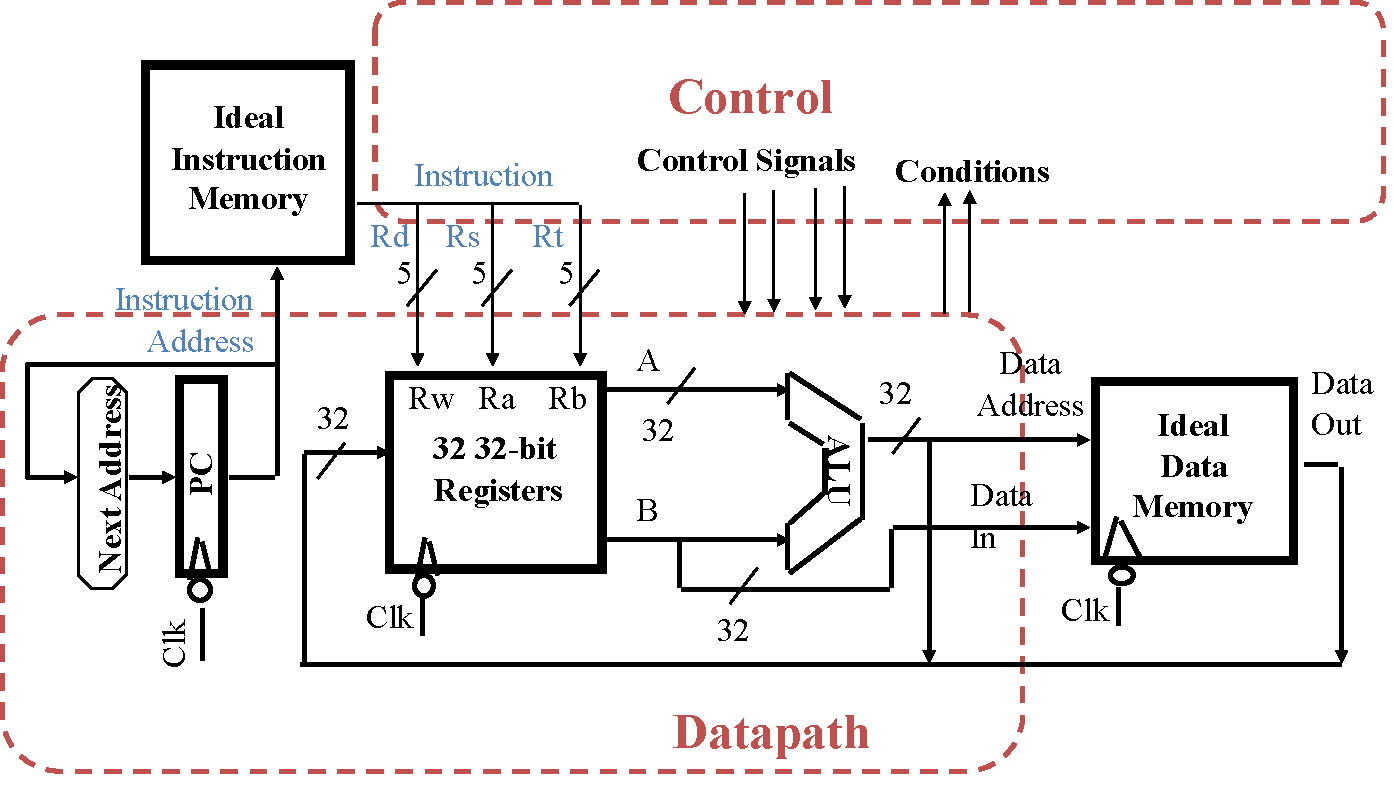
\includegraphics[height=5cm]{images/l1sys.pdf}
 \caption{单周期处理器结构图}
 \label{fig:singleblock}
\end{figure}
如果需要索引参考文献,请使用\cite{Erdos01}, 同时已经将参考文献的项目模版在文末写出。
\subsection{接口定义}\label{sub:Interface}
请详细描述系统顶层接口信号的名称、逻辑特征、时许特性。可以建立类似表\ref{tab:signaldef}这样的列表进行说明。

\begin{table}[htp]
\caption{测试模式信号定义}\label{tab:signaldef}
\begin{center}
	\begin{tabular}{|l|l|l|p{6cm}|}
	\hline
	\textbf{信号名} & \textbf{方向} & \textbf{位宽} & \textbf{功能描述}\\ \hline \hline
	boot			& Input 	& 1-bit	& 触发测试模式, 当处理器正常工作时被置为0\\ \hline
	test\_im\_wr 	& Input	& 1-bit	& Instruction memory write enable in test mode,set to 0 in 	
								  CPU regular process mode. In test mode, it will be set to 1 when if writing instructions to imem, otherwise it is set to 0.\\ \hline
	test\_im\_re 	& Input & 1-bit & Instruction memory read enable in test mode,set to 0 in 	
								  CPU regular process mode. In test mode, it will be set to 1 when if reading instructions out, otherwise it is set to 0. \\ \hline
	test\_im\_addr 	& Input & 32-bit& Instruction memory address\\ \hline
	test\_im\_in 	& Input & 32-bit& Instruction memory data input for test mode. \\ \hline
	test\_im\_out 	& Output& 32-bit& Instruction memory data output for test mode. \\ \hline
	test\_dm\_wr 	& Input	& 1-bit	& Data memory write enable in test mode,set to 0 in 	
								  CPU regular process mode. In test mode, it will be set to 1 when if writing data to dmem, otherwise it is set to 0.\\ \hline
	test\_dm\_re 	& Input & 1-bit & Data memory read enable in test mode,set to 0 in 	
								  CPU regular process mode. In test mode, it will be set to 1 when if reading data out, otherwise it is set to 0.\\ \hline
	test\_dm\_addr 	& Input & 32-bit& Data memory address\\ \hline
	test\_dm\_in 	& Input & 32-bit& Data memory input for test mode. \\ \hline
	test\_dm\_out 	& Output& 32-bit& Data memory output for test mode. \\ \hline
	valid			& Output& 1-bit & If CPU stopped or any exception happens, valid signal is set to 0.\\ 
	\hline
	\end{tabular}
\end{center}
\end{table}

\subsection{接口的(时许)逻辑}\label{sub:logicinter}
请在这个小节描述顶层结构中接口信号使用的逻辑、时序关系等。同样请利用图、表的方法进行描述。特别是时序,请画出时许图。
% -----------------------------------BLOCKS DESIGN----------------------------------------
\section{模块详细设计}
这一节,主要描述各个模块的功能、接口、逻辑控制方法(状态机控制方法)等。
\subsection{ALU}\label{sub:alu}
\subsubsection{功能描述}
\subsubsection{接口定义}
\subsubsection{逻辑控制}

\subsection{控制模块}\label{sub:ctl}
\subsubsection{功能描述}
\subsubsection{接口定义}
\subsubsection{逻辑控制}

\subsection{数据通路}\label{sub:dat}
\subsubsection{功能描述}
\subsubsection{接口定义}
\subsubsection{逻辑控制}

%add more subsections for other block in you CPU design.

\section{实验过程记录}\label{labrec}
记录实验的过程,完成了什么样的工作,存在的问题包括哪些,解决方案如何等。subsubsection名称自行设定。

% -----------------------------------Appendix----------------------------------------
\appendix
\section{代码}\label{sub:app.code}
请在附录\ref{sub:app.code}中添加代码。请使用如下Scala的语法高亮描述方法。
\begin{scala}
class TopIO extends Bundle() {
	val boot = Input(Bool()) 
// imem and dmem interface for Tests
	val test_im_wr		= Input(Bool())
	val test_im_rd 		= Input(Bool())
	val test_im_addr 	= Input(UInt(32.W))
	val test_im_in 		= Input(UInt(32.W))
	val test_im_out 	= Output(UInt(32.W))

	val test_dm_wr		= Input(Bool())
	val test_dm_rd 		= Input(Bool())
	val test_dm_addr 	= Input(UInt(32.W))
	val test_dm_in 		= Input(UInt(32.W))
	val test_dm_out 	= Output(UInt(32.W))

	val valid			= Output(Bool())
}
class Top extends Module() {
	val io 		= IO(new TopIO())//in chisel3, io must be wrapped in IO(...) 
	//...
	when (io.boot & io.test_im_wr){
		imm(io.test_im_addr) := io.test_im_in
		} .elsewhen (io.boot & io.test_dm_wr){
		// please finish it
		} //...
}
\end{scala}
\newpage
% -----------------------------------REFERENCE----------------------------------------
\begin{thebibliography}{9}
\bibitem{Erdos01} P. Erd\H os, \emph{A selection of problems and
results in combinatorics}, Recent trends in combinatorics (Matrahaza,
1995), Cambridge Univ. Press, Cambridge, 2001, pp. 1--6.
\end{thebibliography}
\end{document}

